
%%% Local Variables: 
%%% mode: latex
%%% TeX-master: "main"
%%% End: 

% This section describes the prevalence of the background signal
% Showing specific examples of the background signal and promoter prevalence

\subsubsection{Background Signal}
\begin{wrapfigure}{l}{0.4\textwidth}
\small
\vspace{-20pt}
\begin{center}
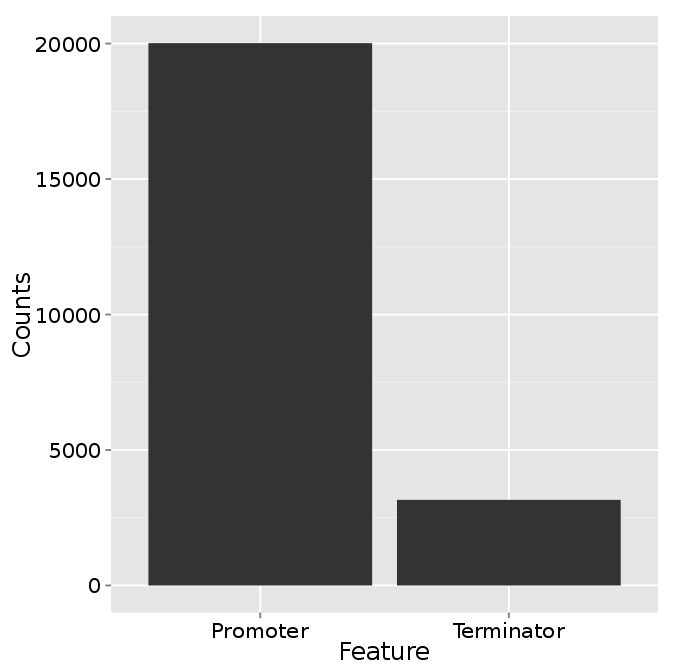
\includegraphics[width=0.38\textwidth]{images/Assembly/Background_signal/prediction_frequency.png}
\caption{Feature Frequency}\label{fig:5.6}
Barplot of total numbers of predicted $\sigma_{A}$-promoters and Rho-independent terminators, indicating the abundance of promoters in the AT-rich \textit{C. acetobutylicum} genome.
\end{center}
\vspace{-20pt}

\end{wrapfigure}

In the previous section, a genome browser and promoter prediction tool were described to facilitate an integrative analysis and curation of the \textit{C. acetobutylicum} genome. In this section, these tools were used to assess the background signals responsible for misassembly, produced from the high sensitivity of this experiment. A large number of Sigma A promoters were predicted (p < 0.01) throughout the \textit{C. acetobutylicum} genome (\ref{fig:5.6}), close to 3x the number of predicted terminators. These promoters were uniformly distributed and perhaps surprisingly, were not necessarily concentrated at the beginning of transcripts (\ref{fig:5.7}). Many of these predictions were weak matches to the consensus motifs (p > 0.001) and would in turn have had only weak affinity for $\sigma$-factors and residual transcriptional activity. The AT-rich genome of \textit{C. acetobutylicum} leads to an abundance of putative promoter sequences, contributing to the background signal observed both statistically and through specific examples (\ref{fig:5.8}). In addition to the previously described benefit of integrating promoter motifs into the curation process, this enabled the quantification of their prevalence and quality. The abundance of $\sigma$_{A} motifs in this AT rich genome could be partially responsible for some of the background signal and misassemblies.

\begin{figure}
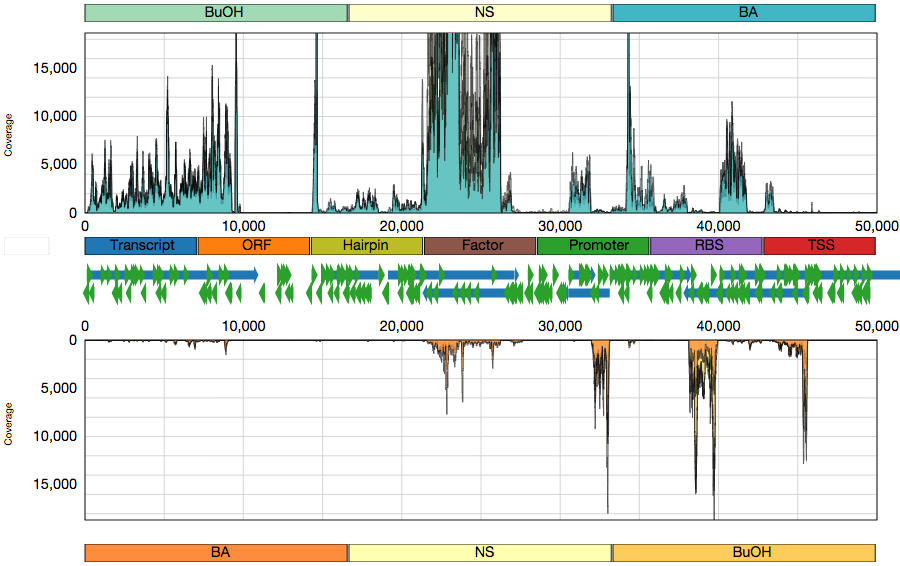
\includegraphics[width=\textwidth]{images/Assembly/Background_signal/promoter_prevalence.png}
\caption{Promoter Prevalence}\label{fig:5.7}
\small
A representative region of the \textit{C. acetobutylicum} genome with a large number of $\sigma_{A}$ promoter motifs relative to the Rho-independent terminators. The high frequency of these promoters in the AT-rich \textit{C. acetobutylicum} genome may contribute to the high background signal.
\end{figure}

\begin{figure}
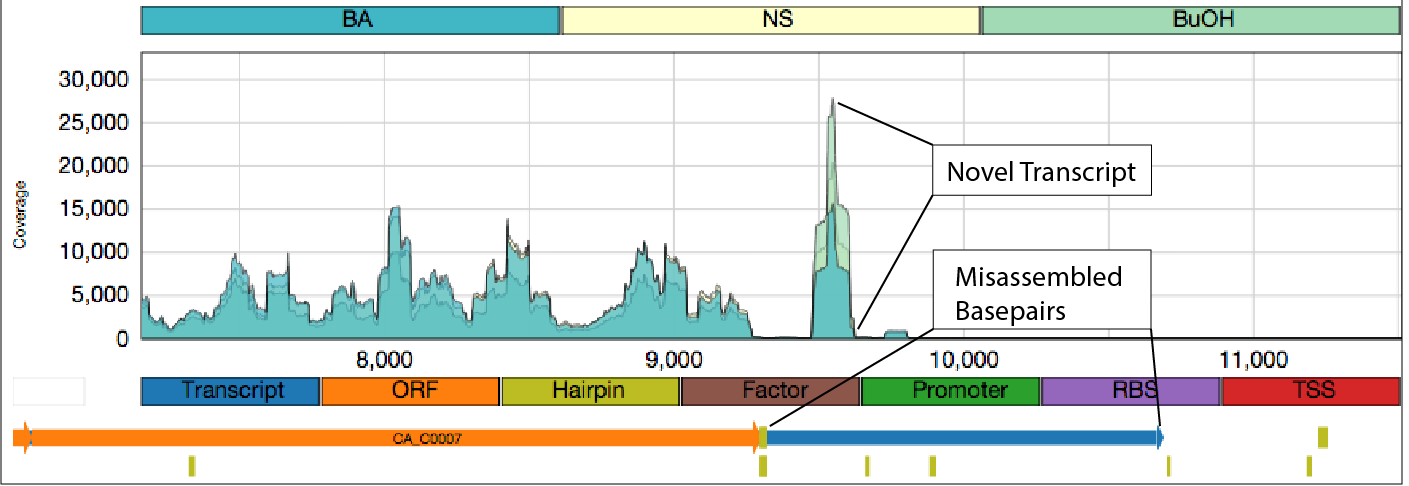
\includegraphics[width=\textwidth]{images/Assembly/Background_signal/Background_signal.png}
\caption{Background Signal}\label{fig:5.8}
\small
An example of a misassembled trancript is shown, extended beyond the hairpin/terminator into the intergenic region. A novel transcript is indicated that may have contributed to this misassembly, although the misassembly extends into obvious troughs of sequencing depth. The misassembled region and novel transcript are indicated in the figure.
\end{figure}

The transcriptome assembly was inspected with the customized genome browser to understand this background signal and determine if the transcript boundary estimates could be improved by curation. The assembled transcripts matched the sequencing depth well, despite the misassemblies that were apparent upon examination (\ref{fig:5.8}). Assembly extended through some troughs in depth (transcript fusion) and beyond expression termini (transcript extension). The extent of background signal - residual depth in seemingly inactive regions of the genome - is impossible to quantify without first distinguishing true signal from the noise through assembly curation. However, background signal is not uncommon with RNA-seq,\cite{110,176,163,164} despite neglect in comparable bacterial studies.

Potential sources for this noise include residual antisense signal (1-5\%), contaminating DNA, and spurious transcription. These signals that were minimized (ref methods) but are difficult to eliminate completely in RNA sequencing experiments(ref background signal papers). Residual antisense signal was not overly abundant(1-5\%), mostly a factor of the library preparation method.\cite{18} Contaminating DNA was minimized and not observed during quality control checkpoints. While these residual contaminants might have contributed towards the background signal, they were expected to be distributed uniformly throughout the genome. These signals could have contributed to the misassembly.

The last source, spurious transcription, can be minimized through certain extraction and size selection techniques during library preparation. However, this experiment was designed to identify all coding and noncoding primary transcripts. The RNA extraction technique used did not exclude short transcripts, such as those from non-specific transcription. The previously described sequencing depth suggested that some of this signal was expected.\cite{110,176,163,164} Spurious transcription was also supported by the promoter prediction frequency (\ref{fig:5.6}) and uniform distribution of these motifs in both transcribed and untranscribed regions of the genome (\ref{fig:5.7}). Similarly to the other noise factors, a small and uniform noise is expected given the extreme sequencing depth, and this noise is a likely cause of misassembly.

Fortunately, there were distinct depth patterns (\ref{fig:5.8}) that agree with promoter and terminator annotations. The separation of true signal from noise was possible by integrating these multiple datasets through the genome browser. Next, the curation process is detailed for specific examples, where previous gene-specific experiments have produced transcript boundaries. The integrated analysis corrected for these background signals, revealing precise and accurate estimates of transcript boundaries. 



